%%%%%%%%%%%%%%%%%%%%%%%%%%%%%%%%%%%%%%%%%
% Short Sectioned Assignment
% LaTeX Template
% Version 1.0 (5/5/12)
%
% This template has been downloaded from:
% http://www.LaTeXTemplates.com
%
% Original author:
% Frits Wenneker (http://www.howtotex.com)
%
% License:
% CC BY-NC-SA 3.0 (http://creativecommons.org/licenses/by-nc-sa/3.0/)
%
%%%%%%%%%%%%%%%%%%%%%%%%%%%%%%%%%%%%%%%%%

%----------------------------------------------------------------------------------------
%	PACKAGES AND OTHER DOCUMENT CONFIGURATIONS
%----------------------------------------------------------------------------------------

\documentclass[paper=a4, fontsize=11pt]{scrartcl} % A4 paper and 11pt font size

\usepackage[T1]{fontenc} % Use 8-bit encoding that has 256 glyphs
\usepackage{fourier} % Use the Adobe Utopia font for the document - comment this line to return to the LaTeX default
\usepackage[english]{babel} % English language/hyphenation
\usepackage{amsmath,amsfonts,amsthm} % Math packages
\usepackage[utf8]{inputenc} %For words with accents

\usepackage{lipsum} % Used for inserting dummy 'Lorem ipsum' text into the template

\usepackage{sectsty} % Allows customizing section commands

\usepackage{graphicx} % Required for including images
\graphicspath{{Figures/}} % Set the default folder for images
\usepackage[hidelinks]{hyperref}

\usepackage{listings} %code interpreter
\lstset{language=Prolog}
\lstset{numbers=left, numberstyle=\small}


\allsectionsfont{\centering \normalfont\scshape} % Make all sections centered, the default font and small caps

\usepackage{fancyhdr} % Custom headers and footers

\pagestyle{fancyplain} % Makes all pages in the document conform to the custom headers and footers
\fancyhead{} % No page header - if you want one, create it in the same way as the footers below
\fancyfoot[L]{} % Empty left footer
\fancyfoot[C]{} % Empty center footer
\fancyfoot[R]{\thepage} % Page numbering for right footer
\renewcommand{\headrulewidth}{0pt} % Remove header underlines
\renewcommand{\footrulewidth}{0pt} % Remove footer underlines
\setlength{\headheight}{13.6pt} % Customize the height of the header

\numberwithin{equation}{section} % Number equations within sections (i.e. 1.1, 1.2, 2.1, 2.2 instead of 1, 2, 3, 4)
\numberwithin{figure}{section} % Number figures within sections (i.e. 1.1, 1.2, 2.1, 2.2 instead of 1, 2, 3, 4)
\numberwithin{table}{section} % Number tables within sections (i.e. 1.1, 1.2, 2.1, 2.2 instead of 1, 2, 3, 4)

\setlength\parindent{0pt} % Removes all indentation from paragraphs - comment this line for an assignment with lots of text

%----------------------------------------------------------------------------------------
%	TITLE SECTION
%----------------------------------------------------------------------------------------

\newcommand{\horrule}[1]{\rule{\linewidth}{#1}} % Create horizontal rule command with 1 argument of height

\title{	
\normalfont \normalsize 
\textsc{Programação em Lógica - FEUP 2018} \\ [25pt] % Your university, school and/or department name(s)
\horrule{0.5pt} \\[0.4cm] % Thin top horizontal rule
\huge Eigenstate \\ % The assignment title
\horrule{2pt} \\[0.5cm] % Thick bottom horizontal rule
}

\author{
	Ricardo Jorge de Araújo Ferreira - up200305418\\
	\normalsize\itshape Grupo Eigenstate\_2\\
	\small Projecto no github: \url{https://github.com/ricardojaferreira/Eigenstate}
} % Your name
%

\date{\normalsize 18 de Novembro de 2018} % Today's date or a custom date

\begin{document}

\maketitle % Print the title

%-----------------------------------
%   Introdução
%-----------------------------------
\section{Introdução}

Neste trabalho foi desenvolvido o jogo Eigenstate \cite{GameGeek:2018}. Eigenstate, é um jogo de tabuleiro para dois jogadores. As regras do jogo e a sua história são apresentadas na secção \ref{ojogo}.

Pretende-se com este trabalho, desensenvolver um jogo que, obdecendo às regras, valide a movimentação das peças e verifique condições de terminação do jogo com derrota, vitória ou empate. Devem ainda ser desenvolvidos os seguintes modos de jogo: Humano/Humano, Humano/Computador, Computador/Humano e Computador/Computador. As jogadas do computador devem ser desenvolvidas com dois modos possíveis. Um modo aleatório, em que cada jogada é escolhida de modo aleatório, sem se preocupar se essa será a melhor jogada naquele momento. No entanto, todas as jogadas devem ser válidas, atendendo às regras do jogo. Outro modo mais avançado, em que, antes de cada jogada, é feita uma validação do estado actual do jogo e escolhida a melhor jogada para aquele estado. Neste jogo, uma jogada envolve, mover uma peça e colocar Pegs em duas peças para permitir mais movimentos em jogadas seguintes. Atendendo a isto, o modo avançado, deve determinar não só a melhor movimentação possível, mas também a colocação de Pegs que potenciem uma melhor futura jogada. No caso aleatório, a colocação de Pegs é também aleatória.

O jogo foi implementado utilizando a linguagem Prolog em SWI-Prolog.

O jogo deve ter também uma interface em modo de texto, que permita ao jogador de forma intuitiva interagir com o jogo e verificar o estado do mesmo.

Todos os objectivos foram cumpridos e todas as regras do jogo implementadas. Nas próximas secções será apresentado em detalhe a lógica do jogo.


%----------------------------------------------------------------------------------------
%	O Jogo Eigenstate
%----------------------------------------------------------------------------------------

\section{O Jogo Eigenstate} \label{ojogo}


\subsection{História}

Eigenstate é um jogo de tabuleiro criado por Martin Grider \cite{GameGeek:2018}. É um jogo para dois jogadores com regras simples mas que cresce em complexidade à medida que o jogo avança. Este jogo ainda não está disponível no mercado, mas prêve-se a criação de um projecto no kickstarter para isso acontecer.

Eigenstate foi inspirado nos jogos The Duke \cite{TheDuke:2013} e Onitama \cite{Onitama:2014}. Durante o seu desenvolvimento o autor escreveu vários cenários de jogabilidade e condições de vitória, tendo pensado até num cenário semelhante ao checkmate do Xadréz. Mas no final, durante uma apresentação do jogo, decidiu manter apenas duas regras básicas. O jogador na sua vez só tem que mover uma peça e colocar dois novos pegs para possibilitar movimentos numa nova jogada. Termina com a eliminação das peças adversárias, no entanto, a condição de vitória ainda pode ser alterada na versão final.

O nome Eigenstate vem de um termo da física quântica que se refere ao possível movimento de uma partícula \cite{Chesstris:2018}.

%----------------------------------------------------------------------------------------
%	Regras
%----------------------------------------------------------------------------------------

\subsection{Regras}

\subsubsection{Configuração}

O jogo joga-se num tabuleiro quadrado com 36 células (6x6). Cada jogador escolhe uma cor e coloca todas as peças dessa cor, 6 peças por jogador, no seu lado do tabuleiro.

Todas as peças começam com dois pegs, um no centro que representa a posição actual da peça e outro peg que permite a peça avançar uma casa.

\begin{figure}[tb]
	\centering
	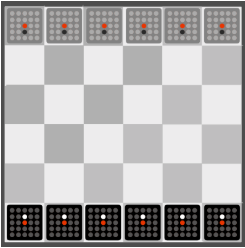
\includegraphics{eigenstate}
	\caption[Eigenstate Setup Inicial]{Eigenstate: Configuração inicial. \cite{eigenstaterules:2018}} % The text in the square bracket is the caption for the list of figures while the text in the curly brackets is the figure caption
	\label{fig:eigenstatestup} 
\end{figure}

\subsubsection{Jogabilidade}

Cada jogador no seu turno, se possível, deve:

\begin{enumerate}
	\item Mover uma das suas peças em conformidade com os pegs (como explicado mais à frente);
	\item Colocar dois pegs em qualquer uma das suas peças, na mesma, ou diferentes.
\end{enumerate}

O movimento das peças é regido pelo seguinte. Todos os pegs colocados na peça representam possíveis jogadas relativamente à sua posição actual. A posição actual é marcada pelo peg colocado no centro, tipicamente com uma cor diferente dos outros.

Este movimento está ilustrado na figura \ref{fig:eigenstatemoves}. Na figura é possível ver que o jogador moveu a peça 1 e colocou dois novos pegs, um na peça que moveu e outro na peça 2. Na próxima jogada, este jogador poderá mover a peça 1 para as posições "a" ou "b" e a peça 2 pode ser colocada nas posições "d" ou "c". Estes movimentos correspondem à posição dos pegs em cada peça.

\begin{figure}[tb]
	\centering
	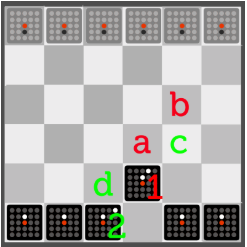
\includegraphics{eigenstate_moves}
	\caption[Eigenstate: Movimento das peças.]{Eigenstate: Movimento de peças. \cite{eigenstaterules:2018}} % The text in the square bracket is the caption for the list of figures while the text in the curly brackets is the figure caption
	\label{fig:eigenstatemoves} 
\end{figure}

O movimento das peças obdece ainda às seguintes regras:

\begin{itemize}
	\item Os pegs nunca podem ser removidos das peças, garantindo que as peças podem sempre avançar uma casa;
	\item As peças podem saltar por cima de outras peças;
	\item As peças não podem sair do tabuleiro;
	\item As peças não rodam;
	\item As peças só se podem mover para trás se tiverem pegs atrás do marcador central;
	\item Uma peça que se mova para a mesma posição de outra peça, faz com que a outra seja removida do tabuleiro;
	\item Peças do mesmo jogador, podem mover-se para cima uma das outras e as peças têm que ser removidas conforme a regra anterior.
\end{itemize}

A colocação de pegs, obdece às seguintes regras:

\begin{itemize}
	\item Só podem ser colocados em espaços livres, das peças do jogador não capturadas;
	\item Em cada turno podem ser colocados 2 pegs em peças diferentes ou na mesma;
	\item Não é necessário colocar nenhum peg na peça movida nessa ronda.
\end{itemize}

\subsubsection{Condição de Vitória}

A forma principal de vitória consiste em reduzir o adversário a apenas uma peça. Num caso em que ambos os jogadores tenham duas peças cada um, a vitória pode ser conseguida se um jogador colocar pegs em todas as posições de uma das suas peças.

%----------------------------------------------------------------------------------------
%	Lógica do Jogo
%----------------------------------------------------------------------------------------

\section{Lógica do Jogo}

A implementação do jogo está organizada do seguinte modo:

\begin{itemize}
	\item \textbf{main.pl} - Neste ficheiro está implementado o predicado \textit{play/0} que dá início ao jogo e os predicados relativos ao ciclo de jogo bem como as chamadas para movimentar peças e adicionar pegs. Este ficheiro é o ponto de entrada da aplicação.
	\item \textbf{utils.pl} - Neste ficheiro encontram-se predicados que desempenham funções básicas, como contar o número de elementos numa Lista de Listas (\textit{countElementsOnMatrix/3}) ou obter a posição X e Y de um elemento numa Lista de Listas (\textit{getMatrixElementPosition/4}), entre outras. Estas funções são utilizadas em várias partes da lógica do jogo.
	\item \textbf{Pasta logic}
	\begin{itemize}
		\item \textbf{board.pl} - Predicados relativos a funções e características do tabuleiro de jogo, por exemplo, o tamanho do tabuleiro (\textit{boardSquareSize/1}) ou obter o valor da célula através da posição (\textit{getBoardCellValue/4}).
		\item \textbf{pieces.pl} - Predicados relativos a funções e características das peças, por exemplo, verificar se peça pertence ao jogador (\textit{checkIfPieceBelongsToPlayer/2}) ou inicializar peças (\textit{initPiecesPlayer/2}).
		\item \textbf{players.pl} - Predicados relativos a acções e características dos jogadores, por exemplo, definir o tipo do jogador (\textit{setPlayer/2}) obter a lista de peças activas do jogador (\textit{getListOfPiecesForPlayer/3}).
		\item \textbf{victory.pl} - Predicado  para verificar se o jogo terminou ou se deve continuar (\textit{game\_over/5}).
		\item \textbf{Pasta ai}
			\begin{itemize}
						\item \textbf{move.pl} - Lógica para escolha da melhor jogada para o modo avançado do computador, (\textit{choosePieceToMoveComputerAI/6}).
						\item \textbf{add\_pegs.pl} - Lógica para escolha da peça e colocação de peg  para o modo avançado do computador, com duas estratégias distintas (\textit{strategyFillPegs/7}), (\textit{strategyGoFurther/7}), orquestradas por (\textit{runPegStrategy/7}). O ciclo de jogo chama esta lógica através do predicado (\textit{addPegToPieceComputerAI/4}).
						\item \textbf{common.pl} - Implementação do predicado (\textit{getBestChoiceByScore/4}), utilizado pela lógica de movimentação e de Pegs para escolher a melhor peça e posição baseada numa lista de pesos.
			\end{itemize}
	\end{itemize}
	 \item \textbf{Pasta cli}
	 	\begin{itemize}
	 				\item \textbf{board\_cli.pl} - Predicados para impressão de estados relacionados com o tabuleiro, por exemplo, visualizar o tabuleiro (\textit{display\_game/2}).
	 				\item \textbf{piece\_cli.pl} - Predicados para impressão de peças, por exemplo, (\textit{printOnePiece/2}).
	 				\item \textbf{player\_cli.pl} - Predicados para interação com o jogador, por exemplo, pedir ao jogador para escolher uma célula para mover a peça (\textit{askPlayerToChooseCell/5}).
	 				\item \textbf{printutils.pl} - Utilitários para as funções de visualização, por exemplo, cores das peças dos jogadores (\textit{playerColor/2}).
	 	\end{itemize}
	 \item \textbf{Pasta loaders}	 	 
	 	\begin{itemize}
	 		\item \textbf{load\_cli.pl} - Consulta todos os ficheiros relacionados com a visualização e interação com a consola de texto.
	 		\item \textbf{load\_logic.pl} - Consulta todos os ficheiros relacionados com lógica do jogo.
		\end{itemize}	 	 	 	 
\end{itemize}

Alguns ficheiros, no final, têm uma secção de testes, feita para testar predicados isoladamente, utilizando estados pré-definidos. Estes testes funcionam um pouco como testes unitários utilizando mocks.


\subsection{Representação do Estado do Jogo}  \label{repjogo}

O jogo terá como representações principais o tabuleiro e a peça. Sendo que as peças são também elas tabuleiros para a colocação de pegs, a representação destes dois elementos será semelhante, embora a forma como se interpretam os resultados seja bastante diferente. Ambos terão uma representação baseada em listas de listas.

A representação inicial do tabuleiro será dada pelo predicado \textit{startBoard/1}.

\begin{lstlisting}
startBoard([
		[1,2,3,4,5,6],
		[0,0,0,0,0,0],
		[0,0,0,0,0,0],
		[0,0,0,0,0,0],
		[0,0,0,0,0,0],
		[7,8,9,10,11,12]
])
\end{lstlisting}

O tabuleiro é uma lista com 6 sub-listas, uma para cada linha do tabuleiro. Com esta estrutura, podemos pesquisar o tabuleiro de uma forma análoga a uma matriz, pesquisando por linha e coluna, tirando partido da divisão das listas em \emph{Head} e \emph{Tail}. 

Tendo em conta esta estrutura, para obter o valor de uma célula do tabuleiro, sabendo a sua posição X (Linha) e a sua posição Y (coluna), podemos utilizar o predicado \textit{getBoardCellValue/4}:

\begin{lstlisting}
getBoardCellValue(Board,PosX,PosY,Value):-
	X1 is PosX-1,
	discardElementsFromList(Board,X1,[Line|_]),
	Y1 is PosY-1,
	discardElementsFromList(Line,Y1,[Value|_]).
\end{lstlisting}

Este predicado elimina linhas do tabuleiro até chegar à linha definida pela posição PosX. Obtendo a linha pretendida, são eliminados os elementos da linha até à PosY, obtendo-se uma lista em que o primeiro elemento (\emph{Head}) é o valor pretendido. Esta particularidade de divisão das listas em \emph{Head} e \emph{Tail} permite utilizar o mesmo predicado de eliminação de elementos, tanto para listas de listas como para listas simples, pois, cada lista dentro de outra lista, pode ser tratada como um elemento simples de uma lista.

O predicado \textit{discardElementsFromList/3} é o seguinte:

\begin{lstlisting}
discardElementsFromList(X,0,X).

discardElementsFromList([_|T],N,Result):-
	N1 is N-1,
	discardElementsFromList(T,N1,Result).
\end{lstlisting}

Este predicado vai recursivamente retirando elementos da lista passada como primeiro argumento e termina quando o valor a obter, passado na variável N, chega a zero, passando para Result os elementos restantes da lista.

Os atómos do tabuleiro têm o seguinte significado:

\begin{itemize}
	\item 0 -  célula vazia;
	\item 1 até 6 - peças do jogador 1;
	\item 7 até 12 - peças do jogador 2.
\end{itemize}

Como cada peça pode ter um estado diferente ao longo do jogo (dependendo do número de pegs que tem) é necessário uma representação individual de cada uma.

A aborgadem para a representação das peças será semelhante à utilizada para o tabuleiro, embora com alguma complexidade acrescida. Cada peça será representada por uma lista com o seguinte formato (peça no estado inicial):

\begin{lstlisting}
startPiecePlayer(
	1, [
			[0,0,0,0,0],
			[0,0,0,0,0],
			[0,0,8,0,0],
			[0,0,1,0,0],
			[0,0,0,0,0]
		]
	).
\end{lstlisting}

O método para percorrer as peças será o mesmo utilizado para o tabuleiro, pois cada peça, é ela própria um tabuleiro. Cada átomo nas peças terá o seguinte significado:

\begin{itemize}
	\item 0 -  célula vazia, pode ser colocado um peg;
	\item 1 - célula com peg;
	\item 8 - célula central que marca a posição da peça no tabuleiro.
\end{itemize}

Um predicado de particular interesse para obter valores das peças é o \textit{getPieceElementsPositions/5}:

\begin{lstlisting}
getPieceElementsPositions(_F,_X,[],P,[P]):-
	!.
	
getPieceElementsPositions(Functor,X,[H|T],[],Pegs):-
	getByLine(Functor,[X,-2,H,NewPegLine]),
	X1 is X+1,
	getPieceElementsPositions(Functor,X1,T,NewPegLine,Pegs).

getPieceElementsPositions(Functor,X,[H|T],PrevPegs,[PrevPegs|Pegs]):-
	getByLine(Functor,[X,-2,H,NewPegLine]),
	X1 is X+1,
	getPieceElementsPositions(Functor,X1,T,NewPegLine,Pegs).
\end{lstlisting}

Por cada linha da peça é chamado o predicado \textit{getByLine/2} com um desvio de -2. Este predicado está definido do seguinte modo:

\begin{lstlisting}
	getByLine(P,LArgs):- G=.. [P|LArgs], G.
\end{lstlisting}

Define um operador univ que pode ser chamado com um dos seguintes predicados \textit{getPegsByLine/4}, \textit{getFutureMovementByLine/4} ou \textit{getEmptySpaceByLine/4}, que permitem obter o número de células ocupadas com pegs, o número de células onde é possível colocar um novo peg e o número de células vazias, respectivamente. O valor de desvio de -2 serve para traduzir as posições da peça em deslocação da peça, ou seja, um peg na posição (1,1) corresponde a um movimento de (-2,-2). Se a peça estiver no tabuleiro na posição (4,3), significa que uma deslocação de (-2,-2) colocará a peça na posição (2,1). Sendo o ponto central das peças a posição (3,3), isto significa que as peças podem efectuar deslocações no tabuleiro entre (-2,-2) e (2,2).

\subsection{Visualização do Tabuleiro}

O tabuleiro numa posição inicial está representado na Figura \ref{fig:initstate}. Pode também ser visto a representção das peças de cada jogador na posição inicial. As peças verdes pertencem ao jodador 1 e as peças vermelhas ao jogador 2.

\begin{figure}[tb]
	\centering
	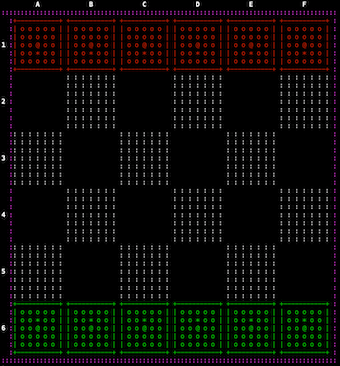
\includegraphics{tabuleiro_init}
	\caption[PROLOG: tabuleiro estado inicial]{Representação do tabuleiro num estado inicial} % The text in the square bracket is the caption for the list of figures while the text in the curly brackets is the figure caption
	\label{fig:initstate} 
\end{figure}

O tabuleiro numa fase de jogo intermédia pode ser visto na Figura \ref{fig:middlestate} e na fase final na Figura \ref{fig:finalstate}.

\begin{figure}[tb]
	\centering
	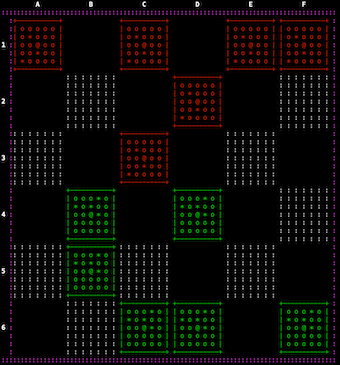
\includegraphics{tabuleiro_middle}
	\caption[PROLOG: tabuleiro estado intermédio]{Representação tabuleiro num estado intermédio} % The text in the square bracket is the caption for the list of figures while the text in the curly brackets is the figure caption
	\label{fig:middlestate} 
\end{figure}

\begin{figure}[tb]
	\centering
	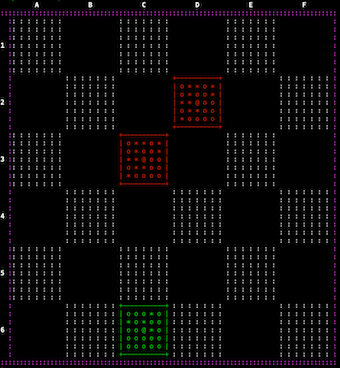
\includegraphics{tabuleiro_final}
	\caption[PROLOG: tabuleiro estado final]{Representação do tabuleiro no estado final.} % The text in the square bracket is the caption for the list of figures while the text in the curly brackets is the figure caption
	\label{fig:finalstate} 
\end{figure}

A Figura \ref{fig:pieceRepresentation} mostra uma peça num estado intermédio do jogo. O símbolo "*" representa Pegs, o símbolo "@" marca a posição actual da peça e o símbolo "O" representa uma célula vazia.

\begin{figure}[tb]
	\centering
	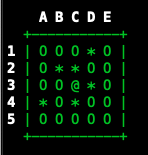
\includegraphics{piece_representation}
	\caption[PROLOG: tabuleiro estado final]{Representação de uma peça num estado intermédio.} % The text in the square bracket is the caption for the list of figures while the text in the curly brackets is the figure caption
	\label{fig:pieceRepresentation} 
\end{figure}


\subsection{Lista de Jogadas Válidas}  \label{validmoves}

Uma jogada válida neste jogo deve respeitar um conjunto de factores, que são: ser uma peça do jogador, ter um peg que lhe permita ir para uma determinada posição e essa posição ser dentro do tabuleiro.

Tendo em vista as condicionantes anteriores, a validação de uma jogada inicia-se com a escolha da peça a mover. No caso de um jogador Humano, essa escolha é feita com o predicado \textit{choosePieceToMove/3}. Este predicado é definido do seguinte modo:

\begin{lstlisting}
choosePieceToMove(Player,Board,PieceToMove):-
	boardSquareSize(S),
	askPlayerToChoosePieceToMove(Player,S,PosX,PosY),
	checkBoardCellChoice(Player,Board,PosX,PosY,PieceToMove),!.
\end{lstlisting}

Verifica-se o tamanho do tabuleiro e pede-se ao jogador para escolher uma posição X e Y dentro do tabuleiro, depois essa posição é validada, para se verificar se representa uma peça do jogador e caso seja, é devolvida a variável \textit{PieceToMove} com o número da peça a mover.

Com esta informação é então possível obter o número de pegs da peça, traduzidos em movimento, como explicado na secção \ref{repjogo} recorrendo ao predicado \textit{getPegsByLine/4}. Pede-se então ao jogador para escolher nova posição X e Y para a colocação da peça e valida-se o movimento com o seguinte predicado:

\begin{lstlisting}
checkIfIsAValidMovement(_Player,PegsPositions,Line,Column,PosX,PosY,PosX,PosY):-
	MovementX is PosX-Line,
	MovementY is PosY-Column,
	checkIfExists([MovementY,MovementX],PegsPositions).

checkIfIsAValidMovement(Player,PegsPositions,Line,Column,_X,_Y,PosX,PosY):-
	showErrorPieceCannotBeMovedToThatLocation,
	getPositionToMove(Player,PegsPositions,Line,Column,PosX,PosY).
\end{lstlisting}

Este predicado recebe o jogador actual, para, caso a peça e movimento escolhido não correspondam a um movimento válido se possa voltar a pedir ao jogador para escolher uma nova opção. Recebe uma lista com a posição, traduzida em movimento, de todos os pegs da peça. Recebe ainda a posição da peça no tabuleiro (Line e Column) e a Posição X e Y para mover a peça (PosX,PosY). Com esta informação é calculado o movimento necessário em X e em Y para a peça ir para a posição escolhida e verifica-se se esse conjunto de movimento existe na lista de Pegs. Caso exista, o movimento é válido, se não, pede-se uma nova opção ao jogador. De notar, que o jogador apenas consegue escolher posições X e Y dentro do tabuleiro, caso não o faça, o predicado \textit{getPositionToMove/6} estará constantemente a ser repetido, pedindo novas posições ao jogador.

Devido a todo este processo iterativo de escolha e validação, este predicado de validação de jogada é único para o jogador humano. No caso do jogador computador (Aleatório ou Avançado) utiliza-se um predicado \textit{valid\_moves/4} mais simples. 

\begin{lstlisting}
valid_moves(Board,Piece,PegsPositions,ValidMoves):-
	getBoardCellPosition(Board,Piece,1,1,Line,Column),
	filterMoves(Line,Column,PegsPositions,ValidMoves),!.
	
filterMoves(_Line,_Column,[],[]).
filterMoves(Line,Column,[[Y,X]|T],[[PosY,PosX]|FT]):-
	PosX is Line+X,
	PosY is Column+Y,
	boardSquareSize(S),
	between(1,S,PosX),
	between(1,S,PosY),
	filterMoves(Line,Column,T,FT).
filterMoves(Line,Column,[_H|T],ValidMoves):-
	filterMoves(Line,Column,T,ValidMoves).
\end{lstlisting}

O computador tem a possibilidade de escolher uma peça a partir de uma lista apenas com peças que pode mover, não havendo necessidade de validar se a peça é do jogador correcto, nem de pedir para escolher nova peça. Do mesmo modo para a escolha do movimento, depois de saber quais os pegs disponíveis, basta filtrar quais os pegs que podem resultar em jogadas válidas e pedir ao computador para escolher uma jogada. O predicado \textit{valid\_moves/4} faz exactamente isso. A partir de uma lista com posições de pegs, traduzidos em movimento, é aplicado um filtro que utiliza a posição da peça escolhida (Line e Column) e obtém-se uma lista de movimentos possíveis para aquela peça (ValidMoves).

O computador pode depois pegar nesta lista e escolher um movimento para executar. Esta escolha irá depender do tipo de computador.

\subsection{Execução de Jogadas}

Como explicado em secções anteriores, uma jogada completa envolve, escolher uma peça para mover, verificar os pegs dessa peça, mover a peça com base nos pegs e escolher peças para colocar dois pegs.

Estes passos são executados no predicado \textit{gameLoop/7} cujo primeiro átomo é um número de 1 a 4 que representa cada um dos estados do movimento:
\begin{itemize}
	\item 1 -  Escolher e mover peça através do predicado \textit{move/6}.
	\item 2 - Escolher peça e adicionar primeiro Peg através do predicado  \textit{playerAddPeg/5}.
	\item 3 - Escolher peça e adicionar segundo Peg através do predicado  \textit{playerAddPeg/5}.
	\item 4 - Responsável por terminar o loop e mostrar o estado final do jogo.
\end{itemize}

Dada a complexidade e condicionantes envolvidas com o movimento de uma peça, o predicado \textit{move/6} terá execuções diferentes, em função do tipo de jogador.

\begin{lstlisting}
move(Player,human,ListOfPieces,Board,NewBoard,NewListOfPieces):-
	choosePieceToMove(Player,Board,PieceToMove),
	movePiece(Player,PieceToMove,ListOfPieces,Board,NewListOfPieces,NewBoard),
	display_game(NewBoard,NewListOfPieces).

move(Player,computerRandom,ListOfPieces,Board,NewBoard,NewListOfPieces):-
	waitForPlayerMove(Player),
	choosePieceToMoveComputer(Player,Board,PieceToMove),
	movePieceComputer(PieceToMove,ListOfPieces,Board,NewListOfPieces,NewBoard),
	display_game(NewBoard,NewListOfPieces).

move(Player,computerAI,ListOfPieces,Board,NewBoard,NewListOfPieces):-
	waitForPlayerMove(Player),
	choosePieceToMoveComputerAI(Player,Board,ListOfPieces,PieceToMove,PosX,PosY),
	movePieceOnBoard(Board,PieceToMove,PosX,PosY,NewBoard),
	updatePieceList(NewBoard,ListOfPieces,NewListOfPieces),
	display_game(NewBoard,NewListOfPieces).
\end{lstlisting}

O jogador humano começa por escolher uma peça para mover (\textit{choosePieceToMove/3}), terminando apenas quando a peça escolhido é uma das suas peças. Sabendo qual a peça a mover, inicia-se a escolha de uma nova posição para a peça, utilizando os predicados de validação apresentados na secção \ref{validmoves}, isto dará origem a um novo tabuleiro (NewBoard), com a posição da peça movida actualizada e uma nova lista de peças (NewListOfPieces), que se poderá manter igual ou ser actualizada, caso tenha sido eliminada alguma peça do tabuleiro. No final mostra-se o tabuleiro resultante.

O jogador computador aleatório, escolhe a peça a mover directamente do tabuleiro, pois sabe quais as peças que lhe pertencem, não precisa de escolher posição X nem Y como o jogador humano. Fazendo então uma escolha aleatório de entre as suas peças, inicia-se o movimento da peça, que consiste na escolha de uma movimentação aleatória escolhida, utilizando o resultado do predicado \textit{valid\_moves/4}, já apresentado. No final, é calculado novo tabuleiro e nova lista de peças como no caso anterior e apresentado o tabuleiro resultante.

O jogador computador avançado, executa funções mais avançadas para a escolha da peça a mover. Estas acções estão descritas nas secções \ref{avtab} e \ref{jogcomp}. Após escolha da peça a mover, o predicado \textit{choosePieceToMoveComputerAI/6} retorna a Peça a mover (PieceToMove) e a posição para onde deve ir a peça (PosX e PosY), que são as mesmas variáveis utilizadas pela movimentação do jogador humano, por isso, no final do movimento do computador avançado, tal como no movimento do jogador humando, os predicados \textit{movePieceOnBoard/5} e \textit{updatePieceList/3} são utilizados para se obter um tabuleiro actualizado e uma nova lista de peças.

Para adicionar novos Pegs é utilizado o predicado \textit{playerAddPeg}, também com execuções diferentes para os diferentes tipos de jogador.

\begin{lstlisting}
playerAddPeg(Player,human,Board,ListOfPieces,NewListOfPieces):-
	addPegToPiece(Player,Board,ListOfPieces,NewListOfPieces),
	display_game(Board,NewListOfPieces).

playerAddPeg(Player,computerRandom,Board,ListOfPieces,NewListOfPieces):-
	waitForPlayerToAddPeg(Player),
	addPegToPieceComputer(Player,Board,ListOfPieces,NewListOfPieces),
	display_game(Board,NewListOfPieces).

playerAddPeg(Player,computerAI,Board,ListOfPieces,NewListOfPieces):-
	waitForPlayerToAddPeg(Player),
	addPegToPieceComputerAI(Player,Board,ListOfPieces,NewListOfPieces),
	display_game(Board,NewListOfPieces).
\end{lstlisting}

A escolha de colocação de pegs será análoga à apresentada para mover uma peça, com a diferença que a posição a escolher será uma posição dentro da peça, não havendo validação de movimentação válida. Deve-se contudo validar que a posição escolhida está vazia e dentro dos limites da peça. O computador aleatório, escolhe uma posição aleatória com base nas posições disponíveis e o computador avançado utiliza um conjunto de regras para decidir qual a melhor posição para colocar o novo peg.

\subsection{Final do Jogo}

O final do jogo pode acontecer de duas formas distintas, um dos jogadores fica reduzido a uma peça e vence o outro jogador, ou ambos os jogadores têm duas peças e vence o primeiro jogador a completar uma peça com pegs.

Para se verificar estas condições em cada fase da movimentação deve-se verificar a condição de vitória, feita através do predicado \textit{game\_over/5}. Este predicado, para além de verificar a condição de vitória, calcula também qual o próximo estado do movimento, como referido na secção \ref{validmoves}.

\begin{lstlisting}
game_over(Loop,Board,_ListOfPieces,NextLoop,Winner):-
	victoryByEatPieces(Board,Loop,NextLoop,Winner).

game_over(Loop,_Board,ListOfPieces,NextLoop,Winner):-
	victoryByPieceWithPegs(ListOfPieces,Loop,NextLoop,Winner).
\end{lstlisting}

O predicado \textit{game\_over/5} utiliza duas estratégias para verificar se o jogo terminou. A primeira é verificar se algum dos jogadores ficou reduzido a apenas uma peça e nesse caso, termina o jogo, devolvendo na variável Winner o vencedor e passando a variável NextLoop para 4. 

Caso não se consiga provar a condição anterior, verifica-se se ambos os jogadores têm apenas duas peças e qual deles tem uma peça com todos os pegs preenchidos. Se isto for provado, o jogo termina, com indicação do vencedor ou empate.

No caso da última validação não se provar, a variável NextLoop é actualizada para o ciclo correspondente e o jogo continua.

\subsection{Avaliação do Tabuleiro} \label{avtab}

A avaliação do tabuleiro é feita através da atribuição de pesos a cada célula do tabuleiro e feita em três fases. Por isso, não se utilizou o predicado \textit{value(+Board, +Player, -Value)} tal como sugerido no enunciado.

Esta avaliação é feita através dos predicados \textit{generateWeightBoard/3}, do predicado \textit{evaluatePiecesAround/6} e \textit{getListOfPiecesAndMovesByScore/5}.

O predicado \textit{generateWeightBoard/3} recebe os átomos List, com a lista de peças do jogador, Board, com o estado actual do tabuleiro e devolve WeightBoard, que será um tabuleiro onde as células têm representados valores correspondentes a pesos, atribuidos com base nos seguintes predicados.

\begin{lstlisting}
weightOfOpponentCells(72).
weightOfEmptyCells(48).
weightOfPlayerCells(0).
\end{lstlisting}

Um tabuleiro de pesos poderá ter o seguinte valor:

\begin{lstlisting}
[
	[72,0,0,48,48,48],
	[48,0,72,48,48,48],
	[48,72,48,48,48,48],
	[48,48,48,48,48,48],
	[48,48,48,48,48,48],
	[48,48,48,48,48,48]
]
\end{lstlisting}

As células do jogador têm um peso de 0, ou seja, representam uma célula sem interesse de movimentação, uma célula vazia, com o valor 48, representa um interesse médio e uma célula com uma peça do adversário com o valor 72, será a mais interessante para mover a peça. Os valores dos pesos foram obtidos considerando que uma peça, no máximo terá 24 posições circundantes com peças do adversário. Fora deste círculo, uma peça adversária já não poderá chegar à peça do jogador, uma vez que, no máximo cada peça se pode mover apenas 2 células. Com o número 24, desenvolveram-se 3 patamares que serão utilizados para o cálculo dos pesos balanceados.

Os pesos balanceados, representam a possibilidade de uma peça em determinada posição poder ser eliminada pelo adversário. Para este cálculo, utiliza-se o predicado \textit{evaluatePiecesAround/6}, que recebe a lista de peças do jogador, a lista de todas as peças em jogo, o tabuleiro, a posição da primeira linha do tabuleiro (na primeira chamada será sempre 1), a lista de pesos calculada anteriormente e devolve uma lista de pesos balanceados, semelhante à seguinte:

\begin{lstlisting}
[
	[71,1,2,47,48,48],
	[48,3,71,48,48,48],
	[47,71,47,47,48,48],
	[47,47,47,47,48,48],
	[47,48,47,48,48,48],
	[48,48,48,48,48,48]
]
\end{lstlisting}

Utilizando a lista de pesos originais, vai ser avaliada, para cada célula, quantas peças adversárias podem, na próxima jogada ir para essa célula. Por cada célula que se possa mover é removido um valor ao peso original, caso a célula em análise represente uma peça vazia ou uma peça do adversário. Se a célula em análise tiver uma peça do jogador, é adicionado um valor por cada peça adversária que se possa mover para essa localização. Deste modo consegue-se representar o real interesse de mover as peças do jogador para determinada posição e quais as pesas do jogador com maior ameaça.

Neste ponto, consegue-se perceber o interesse de ter 3 patamares diferentes de pesos. Sendo que, no máximo poderiam ser possíveis 24 possíveis ataques de peças adversárias para cada célula, consegue-se garantir que uma célula do adversário nunca terá menor interesse que uma célula vazia. Este cenário embora exagerado, pois apenas existem 6 peças por jogador, dá uma noção mais quantitativa do interesse de mover uma peça para determinada posição.

Por fim, o predicado \textit{getListOfPiecesAndMovesByScore/5}, vai organizar, por peça e por jogada, os pesos obtidos com o predicado anterior. Obtendo-se uma lista com o seguinte formato:

\begin{lstlisting}
[
	[Score1,[Piece1,PosX,PosY]],
	[Score2,[Piece1,PosX,PosY]],
	...
]
\end{lstlisting}

Score é a pontuação atribuída a mover a Peça (Piece) para a posição (PosX, PosY). Com esta lista é fácil obter a jogada com a maior pontuação.

Para a escolha das posições para colocar pegs utiliza-se uma estratégia semelhante à de movimentação mas separada por duas estratégias que representam dois estados diferentes do jogo. 

A primeira estratégia, verifica se os jogadores têm apenas 2 peças cada um, nesse caso, a vitória é conseguida preenchendo os pegs numa das peças. Para isto, é utilizado o predicado \textit{strategyFillPegs/5} que vai escolher a peça com o maior número de pegs e avaliar as posições apenas nessa peça.

A segunda estratégia, irá avaliar as jogadas disponíveis em todas as peças, para no final escolher o conjunto peça e posição com a melhor pontuação. Isto é realizado no predicado \textit{strategyGoFurther/5}.

A avaliação da colocação de pegs em determinada posição, é feita com base no tabuleiro de pesos balanceados e calculando qual jogada originará uma maior pontuação, assumindo que o tabuleiro estará na mesma posição quando o jogador voltar a jogar. Este pressuposto, apesar de inválido, não está totalmente errado, uma vez que a jogada do adversário não irá alterar muito o tabuleiro e a colocação de pegs será prioritária para peças não ameaçadas, logo a peça onde se colocar o peg ainda estará no tabuleiro na próxima jogada. Para dar um maior grau de liberdade de movimentação às peças, permitindo deslocações maiores, tanto para escapar como para capturar peças, as posições para coloção de pegs que permitam uma movimentação de duas casas têm um acrescimo de pontuação de 1 valor.

Em caso de empate, tanto para mover peças, como para colocar pegs, é escolhida uma combinação aleatória, dos maiores pesos,  para evitar um padrão nas escolhas do computador.

\subsection{Jogada do Computador} \label{jogcomp}

Novamente, dada a complexidade e o processo iterativo de uma jogada, não é possível descrever todo o processo apenas com um predicado \textit{choose\_move(+Board, +Level, -Move)} tal como sugerido.

As jogadas do computador são o resultado de todas as validações apresentadas anteriormente. Escolha da peça, movimento, escolha de peças e de posições para colocar pegs. Todas estas movimentações são realizadas pelo predicado \textit{gameLoop/7}, que é chamada logo após as inicializações do jogo e continua em ciclo até o jogo terminar.

\begin{lstlisting}
gameLoop(1,Player,P1Type,P2Type,ListOfPieces,Board,_W):-
	getCurrentPlayerType(Player,P1Type,P2Type,Type),
	move(Player,Type,ListOfPieces,Board,BoardMove,ListOfPiecesMove),
	game_over(1,BoardMove,ListOfPiecesMove,NextLoop,Winner),
	gameLoop(NextLoop,Player,P1Type,P2Type,ListOfPiecesMove,BoardMove,Winner).

gameLoop(2,Player,P1Type,P2Type,ListOfPieces,Board,_W):-
	getCurrentPlayerType(Player,P1Type,P2Type,Type),
	playerAddPeg(Player,Type,Board,ListOfPieces,ListOfPiecesPeg),
	game_over(2,Board,ListOfPiecesPeg,NextLoop,Winner),
	gameLoop(NextLoop,Player,P1Type,P2Type,ListOfPiecesPeg,Board,Winner).

gameLoop(3,Player,P1Type,P2Type,ListOfPieces,Board,_W):-
	getCurrentPlayerType(Player,P1Type,P2Type,Type),
	playerAddPeg(Player,Type,Board,ListOfPieces,ListOfPiecesLastPeg),
	game_over(3,Board,ListOfPiecesLastPeg,NextLoop,Winner),
	nextPlayer(Player,NextPlayer),
	gameLoop(NextLoop,NextPlayer,P1Type,P2Type,ListOfPiecesLastPeg,Board,Winner).

gameLoop(4,_P,_T1,_T2,_LP,_B,Winner):-
	print_gameOver_message(Winner).
\end{lstlisting}

O Loop 1 encarrega-se de escolher e mover a peça, verifica se após a movimentação o jogo terminou e chama o próximo loop. O Loop 2, adiciona o primeiro peg numa peça, verifica se o jogo terminou e chama o próximo loop. O Loop 3, adiciona o segundo peg numa peça, verifica se o jogo terminou, actualiza o próximo jogador e chama o loop 1 caso o jogo não tenha terminado. Por fim, o Loop 4, é chamado caso o jogo termine e imprime uma mensagem com o jogador que ganhou.

\section{Conclusões}

O desenvolvimento deste trabalho, permite concluir que a linguagem Prolog é bastante eficiente para desenvolver sistemas com inteligência artifial. Sendo uma linguagem baseada em lógica, a forma de pensar de um humano é rapidamente traduzida na linguagem.

O desenvolvimento do trabalho foi também bastante enriquecedor, pois permitiu desenvolver uma forma de pensar em programação diferente da tradicional. Foi um desafio no início, mas com o desenrolar do trabalho tornou-se mais natural pensar em lógica e colocar de lado de lado um pensamento mais imperativo de realizar as diferentes accões e obter os objectivos.

É também interessante de avaliar a quantidade de código escrita, que é bastante reduzida quando comparada com outras linguagens.

Em termos de melhorias, pode-se apontar uma maior robustez na forma como os inputs são tratados, uma melhor interface com o utilizador e uma maior quantidade de testes para aumentar a fiabilidade dos predicados e prever mais situações.




%----------------------------------------------------------------------------------------
%	BIBLIOGRAPHY
%----------------------------------------------------------------------------------------
\renewcommand{\refname}{\spacedlowsmallcaps{Referências}} 
\bibliographystyle{unsrturl}
\nocite{swiPrologManual:2018}
\nocite{learnProlog:2012}
\bibliography{sample.bib}


\end{document}